\documentclass[final]{beamer}
\mode<presentation>{\usetheme{ParisSaclay}}

\usepackage[english]{babel}
\usepackage[utf8]{inputenc}
\usepackage[T1]{fontenc}
\usepackage{lmodern}
\usepackage{amsmath,amssymb,amsfonts}
\usepackage{booktabs}
\usepackage{array}
\usepackage{graphicx}
\usepackage{tikz}
\usetikzlibrary{positioning}
\usepackage[orientation=portrait,size=a0,scale=1.34]{beamerposter}

\graphicspath{{./}{../}}
\boldmath

\title{End-to-End Portfolio Optimization with CNN-GARCH}
\author{Wacil Lakbir, Sneha Basker}
\institute{MSc AI Lab Project \quad|\quad Supervisor: Christian Bongiorno\\Contacts: \texttt{[add-wacil-email]} \quad|\quad \texttt{[add-sneha-email]}}

\newlength{\sepwidth}
\newlength{\colwidth}
\setlength{\sepwidth}{0.024\paperwidth}
\setlength{\colwidth}{0.464\paperwidth}

\newcommand{\separatorcolumn}{\begin{column}{\sepwidth}\end{column}}

\begin{document}

\begin{frame}[t]
\begin{columns}[t,totalwidth=\textwidth]

\separatorcolumn

\begin{column}{\colwidth}

\begin{block}{1. Motivation, Research Problem, and Contributions}
\small
\textbf{Motivation}
Global Minimum Variance (GMV) portfolios are highly sensitive to estimation noise:
unstable marginal volatilities and noisy rolling correlations create fragile inverse-covariance weights.

\textbf{Research problem}
Can we improve out-of-sample GMV stability by learning a better covariance-estimation pipeline
while keeping the downstream optimizer fixed?

\begin{center}
\begin{tikzpicture}[node distance=0.75cm,>=stealth,scale=1.0, every node/.style={transform shape}]
\node[draw,rounded corners,fill=psprunelight,minimum width=3.1cm,minimum height=1.25cm,align=center] (r) {\textbf{Returns}\\90-day windows};
\node[draw,rounded corners,fill=psprunelight,right=of r,minimum width=3.2cm,minimum height=1.25cm,align=center] (v) {\textbf{CNN-GARCH}\\\(\hat{\sigma}_t^2\)};
\node[draw,rounded corners,fill=psprunelight,right=of v,minimum width=3.1cm,minimum height=1.25cm,align=center] (c) {\textbf{RIENet}\\cleaned \(C_t\)};
\node[draw,rounded corners,fill=psprunelight,right=of c,minimum width=2.8cm,minimum height=1.25cm,align=center] (w) {\textbf{GMV}\\\(w_t^\star\)};
\draw[thick,psprune,->] (r) -- (v);
\draw[thick,psprune,->] (v) -- (c);
\draw[thick,psprune,->] (c) -- (w);
\end{tikzpicture}
\end{center}

\textbf{Main contributions}
\begin{itemize}
\item a \textbf{hybrid CNN-GARCH} model for marginal volatility forecasting,
\item a \textbf{stable} \((\omega,C,\rho)\) parameterization,
\item a \textbf{RIENet} layer for rolling correlation cleaning,
\item a fair GMV comparison where only the covariance estimate changes.
\end{itemize}

\textbf{Evaluation logic}
\begin{itemize}
\item first reduce \textbf{portfolio volatility},
\item then compare \textbf{Sharpe ratio}.
\end{itemize}
\end{block}

\begin{block}{2. Data Cleaning and Experimental Setup}
\small
\textbf{Dataset:} WIKI adjusted prices from 2000-01-04 to 2018-03-27.

\textbf{Cleaning rules}
\begin{itemize}
\item remove zero-volume observations,
\item compute adjusted-close returns,
\item keep only series complete over the training timeline,
\item exclude low-price stocks using a \(\$3\) threshold on the first test day,
\item exclude assets with more than 20 consecutive zero returns.
\end{itemize}

\textbf{Final setup}
\begin{itemize}
\item 1338 cleaned stocks in the full universe,
\item 50 stocks in the end-to-end GMV poster experiment,
\item 70\% train / 30\% test split,
\item train-only normalization to avoid leakage.
\end{itemize}

\textbf{Why the cleaning matters}
\begin{itemize}
\item low-price and stale-trading stocks create unstable returns,
\item incomplete histories create biased covariance estimates,
\item the filtered universe is designed for robust out-of-sample testing.
\end{itemize}
\end{block}

\begin{block}{3. CNN-GARCH Architecture}
\small
\textbf{Input:} one 90-day return window per stock.

\textbf{Architecture}
\begin{itemize}
\item 5 Conv1D layers,
\item kernel size \(3\),
\item same padding,
\item dilations \(1,2,4,8,16\),
\item GroupNorm + LeakyReLU,
\item global average pooling + dense prediction head.
\end{itemize}

\textbf{Effective receptive field}
\[
\mathrm{RF} = 1 + (k-1)\sum_{i=0}^{4} 2^i
            = 1 + 2(1+2+4+8+16) = 63.
\]

So the convolutional stack directly captures \textbf{63 days} of temporal context,
while the pooled representation still summarizes the full \textbf{90-day window}.

\begin{center}
\begin{tikzpicture}[>=stealth,node distance=1.4mm]
  \tikzset{
    archbox/.style={
      draw,
      rounded corners,
      fill=psprunelight,
      minimum width=1.22cm,
      minimum height=0.78cm,
      align=center,
      inner sep=1.3pt,
      font=\scriptsize
    }
  }
  \node[archbox] (in) {Input};
  \node[archbox,right=of in] (c1) {Conv\\1};
  \node[archbox,right=of c1] (c2) {Conv\\2};
  \node[archbox,right=of c2] (c3) {Conv\\3};
  \node[archbox,right=of c3] (c4) {Conv\\4};
  \node[archbox,right=of c4] (c5) {Conv\\5};
  \node[archbox,right=of c5] (dense) {Dense};
  \node[archbox,right=of dense] (garch) {GARCH};
  \foreach \a/\b in {in/c1,c1/c2,c2/c3,c3/c4,c4/c5,c5/dense,dense/garch} {
    \draw[thick,psprune,->] (\a.east) -- (\b.west);
  }
\end{tikzpicture}
\end{center}
\end{block}

\begin{block}{4. Stable GARCH Parameterization}
\small
Instead of predicting \(\alpha\) and \(\beta\) directly, the network predicts:
\[
\omega = \mathrm{softplus}(h_\omega),\qquad
C = 0.99\,\sigma(h_C),\qquad
\rho = \sigma(h_\rho).
\]

Then:
\[
\alpha = C\rho,\qquad
\beta = C(1-\rho).
\]

\textbf{Why this is useful}
\begin{itemize}
\item \(C\) is constrained between 0 and 1,
\item \(\rho\) is constrained between 0 and 1,
\item therefore \(\alpha,\beta \in (0,1)\),
\item and \(\alpha + \beta = C < 1\), which stabilizes persistence.
\end{itemize}

\textbf{Differentiable GARCH layer}
\[
\hat{\sigma}_{t+1}^2 = \omega + \alpha r_t^2 + \beta \hat{\sigma}_t^2.
\]
The CNN learns the parameters, and the GARCH recursion computes the next variance.
\end{block}

\begin{block}{5. Training Strategy}
\small
\textbf{Stage 1: synthetic pretraining.}
The model first learns generic GARCH dynamics on many simulated GARCH(1,1) series.

\textbf{Stage 2: fine-tuning on real equities.}
It is then adapted to filtered WIKI returns with train-only normalization, zero-aware sampling,
an \(r^2\) floor, and validation-based checkpoint selection.

\textbf{Loss}
\[
\mathcal{L} = \mathrm{MSE}\bigl(\log \sigma_{\text{true}}^2,\log \hat{\sigma}^2\bigr).
\]

\begin{center}
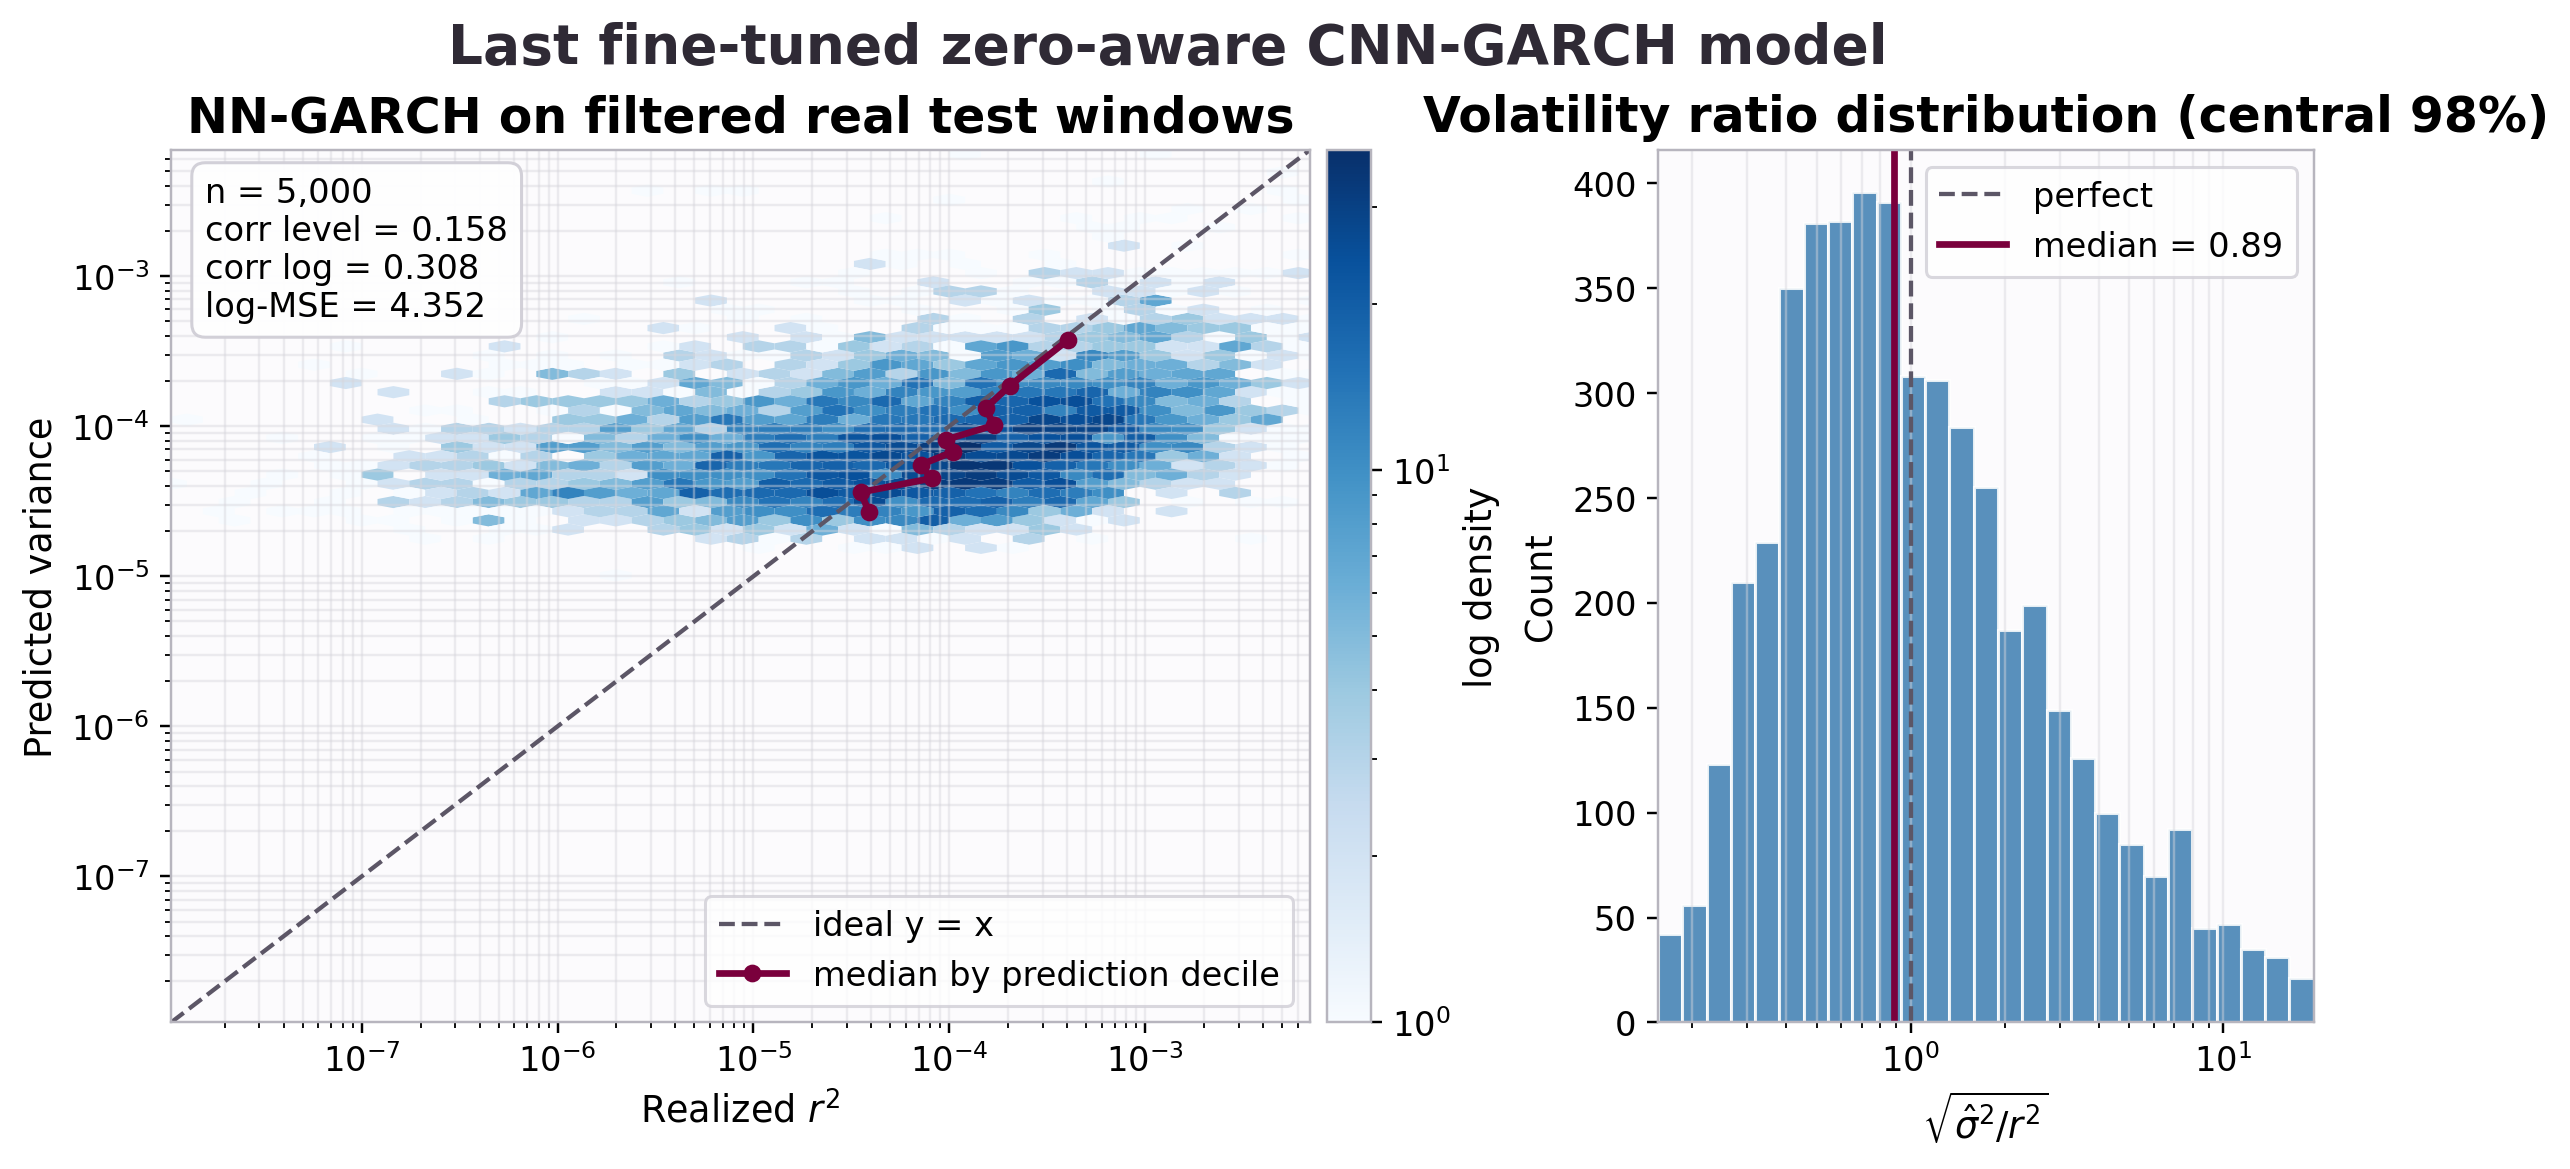
\includegraphics[width=0.74\linewidth]{nn_garch_real_test_diagnostic.png}
\end{center}
\textbf{Figure 1.} Real filtered OOS windows: prediction density and volatility-ratio distribution.
\end{block}
\end{column}

\separatorcolumn

\begin{column}{\colwidth}

\begin{block}{6. RIENet Correlation Cleaning}
\small
\textbf{Motivation}
Rolling sample correlations are noisy. That noise propagates directly to \(\Sigma_t^{-1}\)
and makes GMV weights unstable.

\textbf{RIENet layer explanation}
\begin{enumerate}
\item eigen-decompose the rolling correlation matrix,
\item enrich the eigenvalue sequence with dimension-aware information such as \(q=T/N\) and lookback length,
\item clean the spectrum in inverse-eigenvalue space with a recurrent transform,
\item reconstruct a cleaned correlation matrix.
\end{enumerate}

\textbf{Interpretation}
\begin{itemize}
\item CNN-GARCH estimates the \textbf{marginal variances},
\item RIENet cleans the \textbf{dependence structure},
\item together they produce a more stable covariance matrix.
\end{itemize}

\[
\Sigma_t = D_t\,C_t\,D_t,
\qquad
w_t^\star = \frac{\Sigma_t^{-1}\mathbf{1}}{\mathbf{1}^{\top}\Sigma_t^{-1}\mathbf{1}}.
\]
\end{block}

\begin{exampleblock}{7. Related Work, GMV Construction, and Baselines}
\small
\textbf{Related work}
Classical GMV relies on rolling sample covariance and GARCH-style volatility models.
Covariance cleaning literature uses shrinkage and random-matrix denoising,
and recent end-to-end portfolio optimization papers motivate learning better inputs to the optimizer
instead of changing the allocation rule.

\textbf{Covariance model}
\[
\Sigma_t = D_t C_t D_t
\]
with \(D_t = \mathrm{diag}(\hat{\sigma}_{1,t},\ldots,\hat{\sigma}_{N,t})\).

\textbf{Unconstrained GMV}
\[
w_t^\star = \frac{\Sigma_t^{-1}\mathbf{1}}{\mathbf{1}^{\top}\Sigma_t^{-1}\mathbf{1}}.
\]

\textbf{Methods compared}
\begin{itemize}
\item \textbf{GMV-GARCH}: GARCH volatilities + raw rolling correlation,
\item \textbf{GMV-NN}: CNN-GARCH volatilities + raw rolling correlation,
\item \textbf{GMV-NN-Clean}: CNN-GARCH volatilities + RIENet-cleaned correlation.
\end{itemize}

\textbf{Fair comparison}
All three methods use the same stocks, the same lookback window, and the same GMV formula.
Only the covariance estimate changes.
\end{exampleblock}

\begin{exampleblock}{8. Main Out-of-Sample Results}
\small
\textbf{50-stock unconstrained GMV experiment, 2012--2018}

\begin{center}
\begin{tabular}{>{\raggedright\arraybackslash}p{0.37\linewidth}ccc}
\toprule
Method & Ann. Ret. & Ann. Vol. & Sharpe \\
\midrule
GMV-GARCH & 17.39\% & 13.95\% & 1.2468 \\
GMV-NN & \textbf{20.43\%} & 14.40\% & \textbf{1.4190} \\
GMV-NN-Clean & 17.53\% & \textbf{12.75\%} & 1.3755 \\
\bottomrule
\end{tabular}
\end{center}

\begin{center}
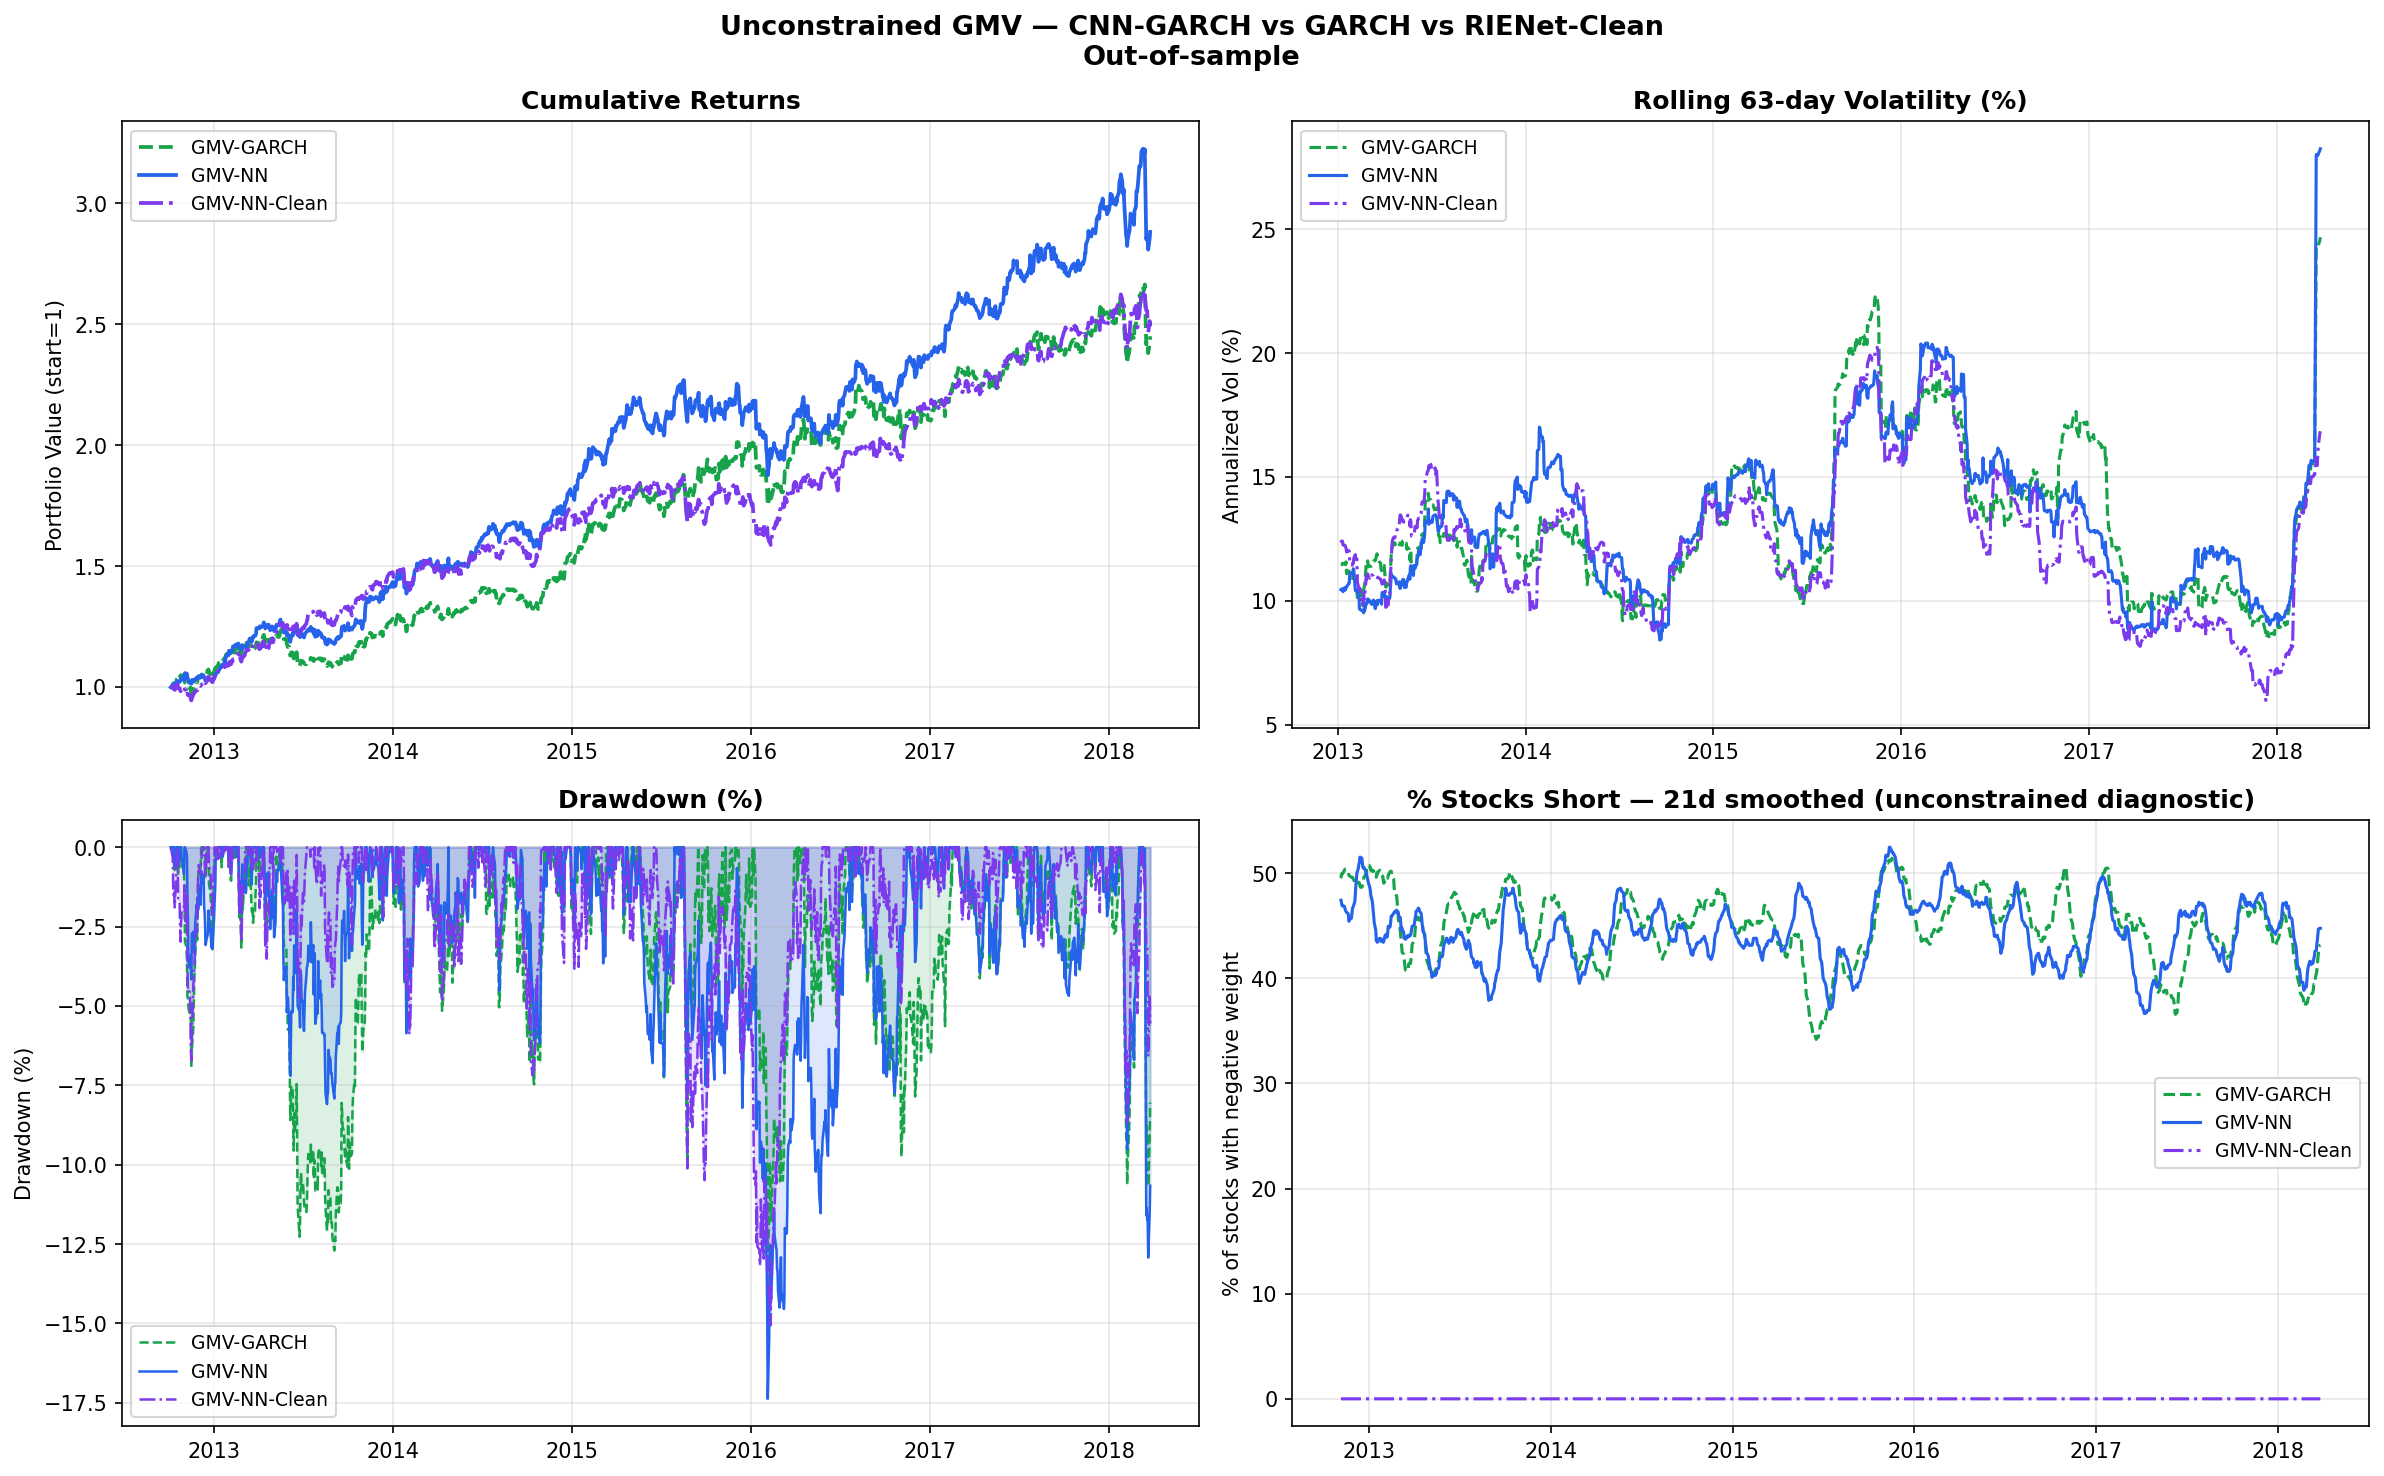
\includegraphics[width=0.99\linewidth]{gmv_unconstrained_results.png}
\end{center}
\textbf{Figure 2.} Cumulative return, rolling volatility, drawdown, and short-weight diagnostic.
\end{exampleblock}

\begin{alertblock}{9. Conclusion, Discussion, and Perspectives}
\footnotesize
\textbf{Discussion}
\begin{itemize}
\item GMV-NN-Clean gives the \textbf{lowest out-of-sample volatility}.
\item GMV-NN gives the \textbf{highest Sharpe ratio}.
\item RIENet cleaning regularizes spectral inversion and reduces fragile allocations.
\end{itemize}

\textbf{Robustness}
On 200 random 30-stock subsets, NN-GARCH also improves average volatility and Sharpe,
and Wilcoxon signed-rank tests are significant for both metrics.

\textbf{Perspectives}
\begin{itemize}
\item scale beyond 50 assets and include transaction costs or long-only constraints,
\item jointly train volatility and correlation modules end-to-end,
\item study turnover regularization and alternative risk objectives.
\end{itemize}

\textbf{Take-away}
\[
\hat{\sigma}^2 \uparrow \text{ quality}
\;+\;
C_t \uparrow \text{ quality}
\Longrightarrow
\Sigma_t \uparrow \text{ quality}
\Longrightarrow
\]
\[
\Longrightarrow
\text{more stable GMV portfolios.}
\]
\begin{center}
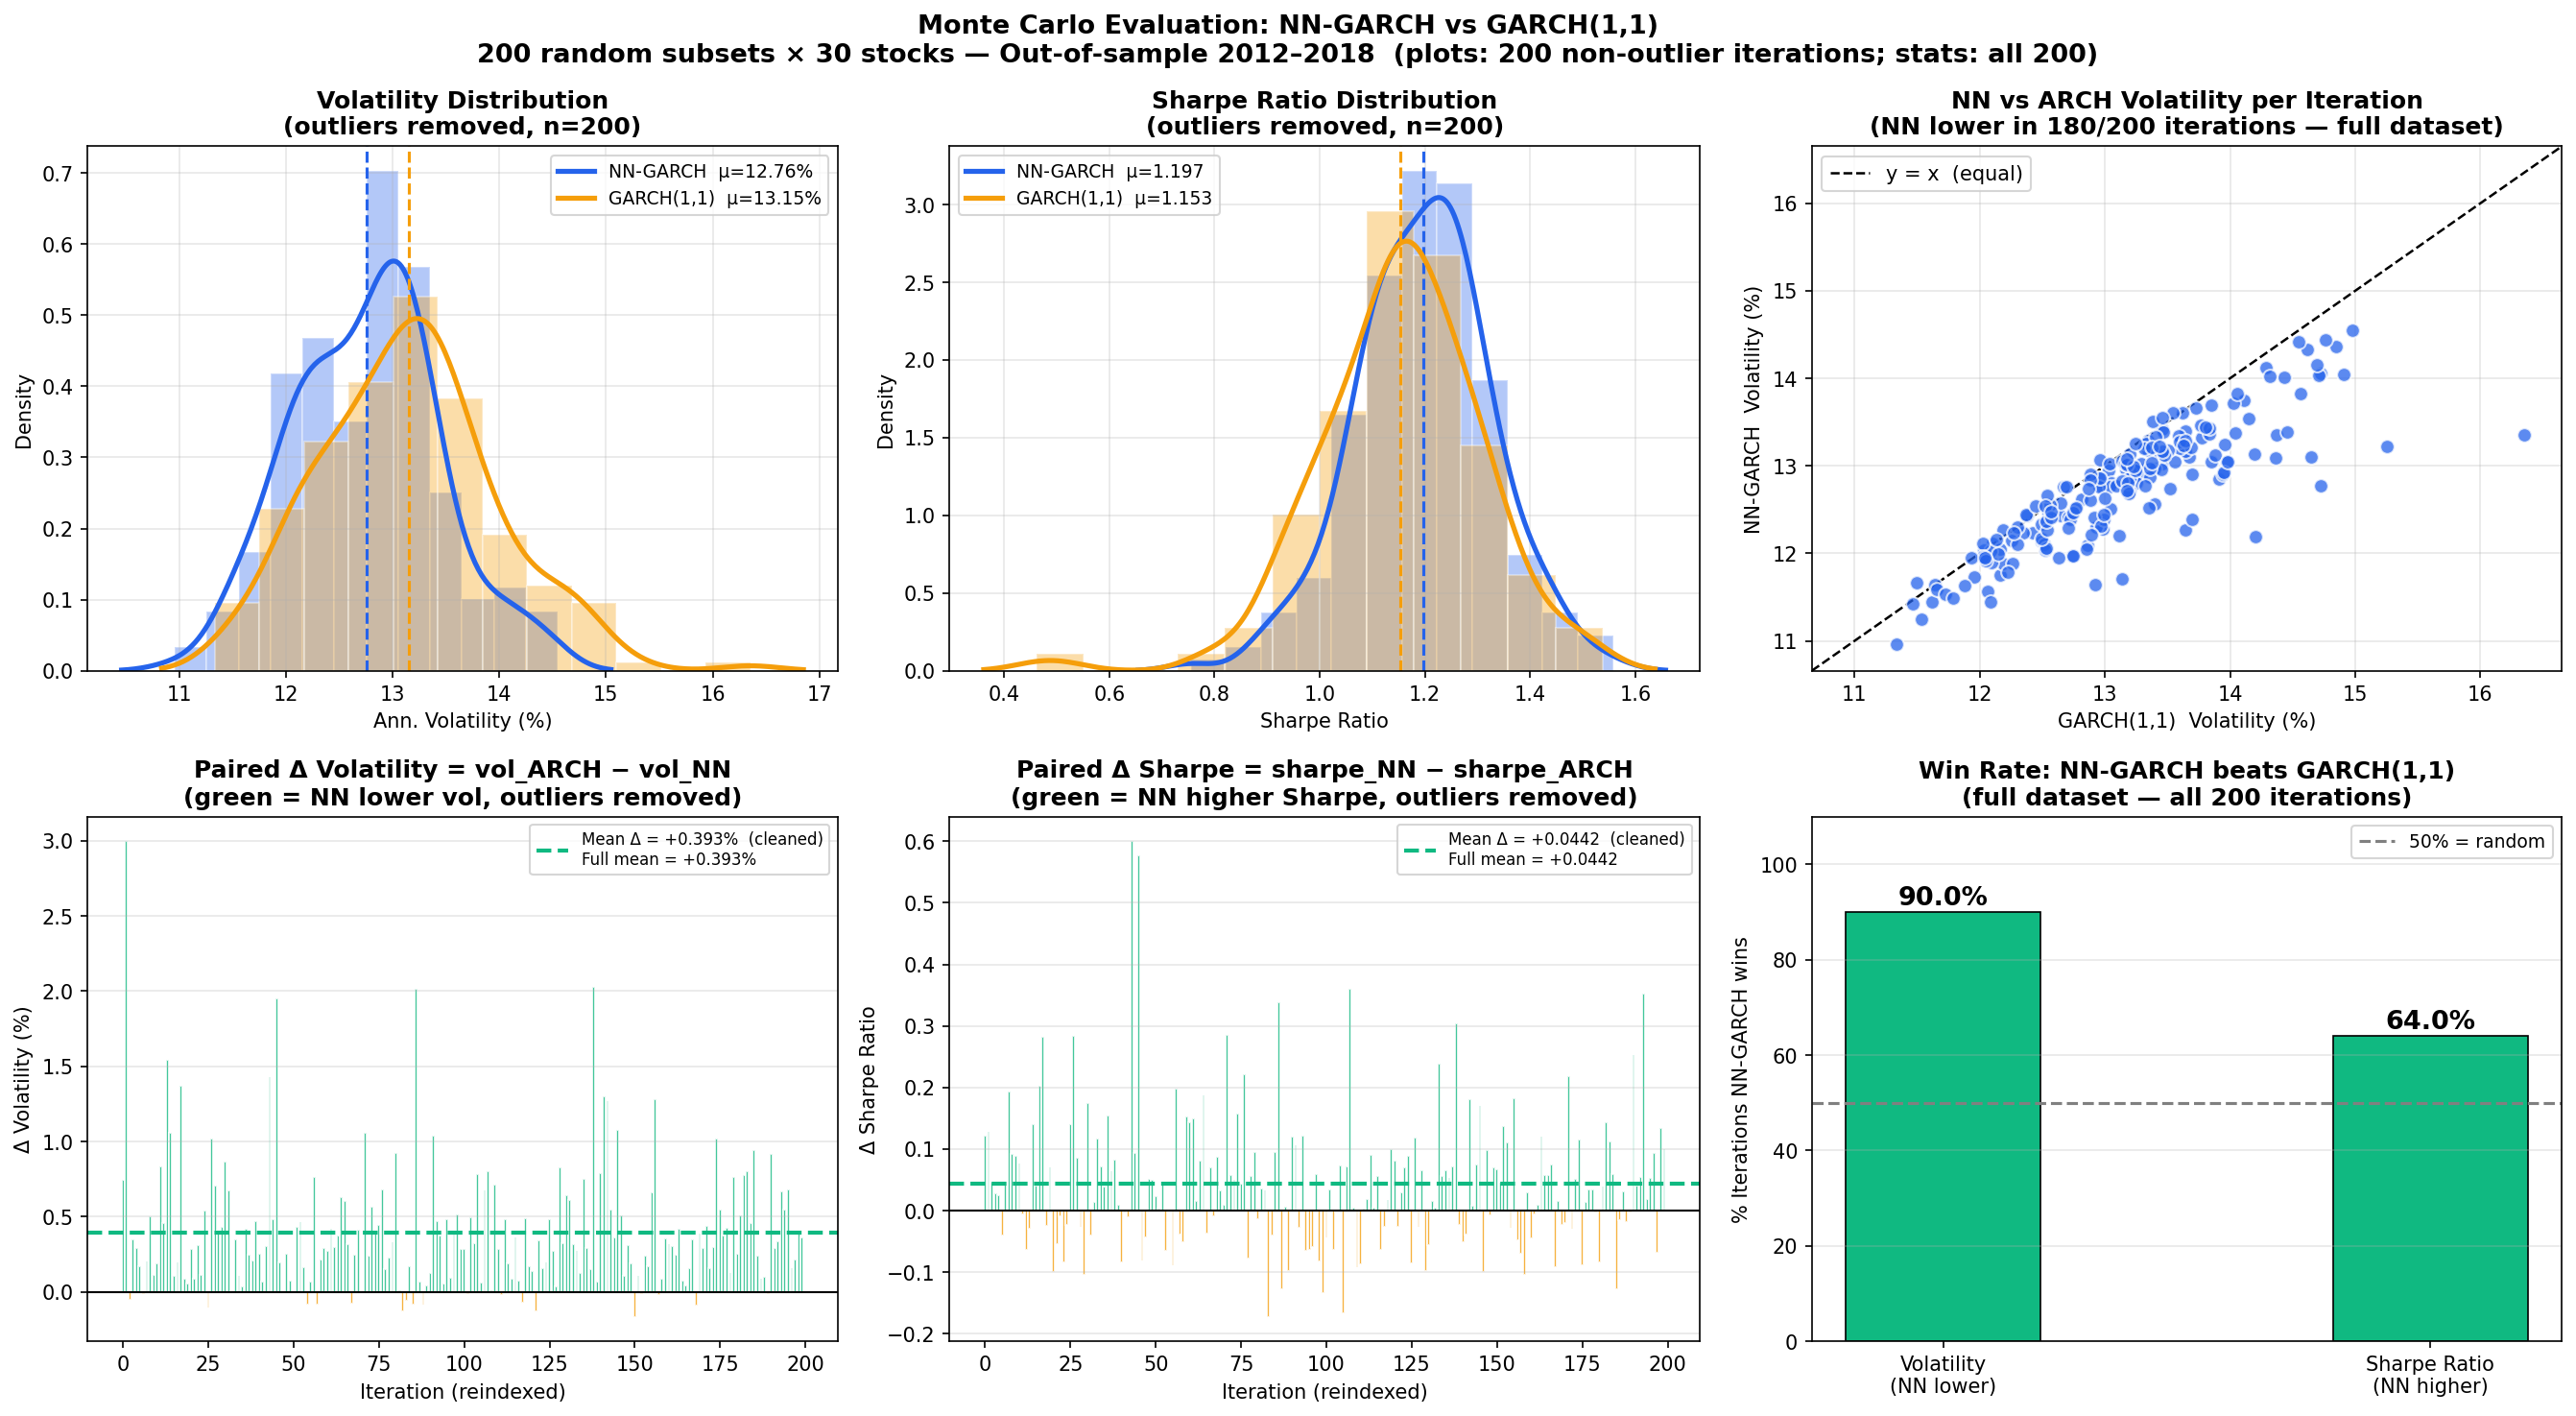
\includegraphics[width=0.90\linewidth]{mc_wilcoxon_distributions.png}
\end{center}
\textbf{Figure 3.} Monte Carlo paired comparisons support the robustness of the learned volatility model.

{\scriptsize
\textbf{Essential references}
\begin{itemize}
\item Bollerslev (1986), \emph{Generalized Autoregressive Conditional Heteroskedasticity}.
\item Ledoit and Wolf (2004), \emph{A Well-Conditioned Estimator for Large-Dimensional Covariance Matrices}.
\item Bongiorno et al. (2025), \emph{End-to-End Large Portfolio Optimization}.
\end{itemize}
}
\end{alertblock}
\end{column}

\separatorcolumn

\end{columns}
\end{frame}

\end{document}
